\documentclass{standalone}
\usepackage{tikz}
\usetikzlibrary{patterns, positioning}


\begin{document}
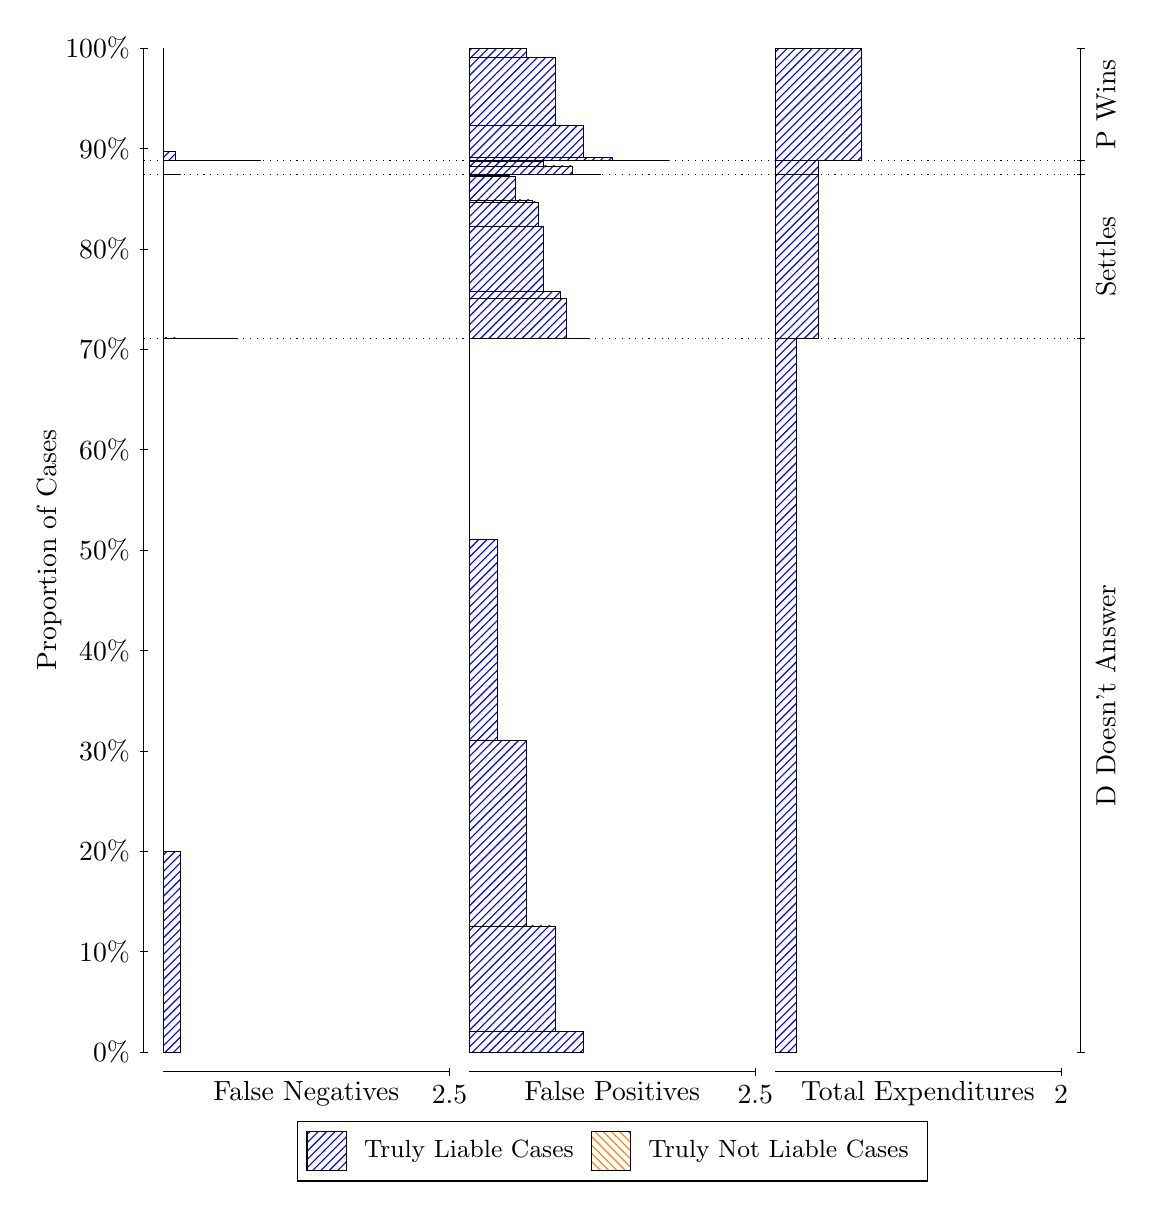
\begin{tikzpicture}
\draw[black, very thin] (1.5,1.75) -- (1.5,14.5);
\node[rotate=90, text=black, anchor=center] at (0.3, 8.125) {Proportion of Cases};
\draw[black, very thin] (1.45,1.75) -- (1.55,1.75);
\node[text=black, anchor=east] at (1.45, 1.75) {0\%};
\draw[black, very thin] (1.45,3.025) -- (1.55,3.025);
\node[text=black, anchor=east] at (1.45, 3.025) {10\%};
\draw[black, very thin] (1.45,4.3) -- (1.55,4.3);
\node[text=black, anchor=east] at (1.45, 4.3) {20\%};
\draw[black, very thin] (1.45,5.575) -- (1.55,5.575);
\node[text=black, anchor=east] at (1.45, 5.575) {30\%};
\draw[black, very thin] (1.45,6.85) -- (1.55,6.85);
\node[text=black, anchor=east] at (1.45, 6.85) {40\%};
\draw[black, very thin] (1.45,8.125) -- (1.55,8.125);
\node[text=black, anchor=east] at (1.45, 8.125) {50\%};
\draw[black, very thin] (1.45,9.4) -- (1.55,9.4);
\node[text=black, anchor=east] at (1.45, 9.4) {60\%};
\draw[black, very thin] (1.45,10.675) -- (1.55,10.675);
\node[text=black, anchor=east] at (1.45, 10.675) {70\%};
\draw[black, very thin] (1.45,11.95) -- (1.55,11.95);
\node[text=black, anchor=east] at (1.45, 11.95) {80\%};
\draw[black, very thin] (1.45,13.225) -- (1.55,13.225);
\node[text=black, anchor=east] at (1.45, 13.225) {90\%};
\draw[black, very thin] (1.45,14.5) -- (1.55,14.5);
\node[text=black, anchor=east] at (1.45, 14.5) {100\%};

\draw[black, very thin] (13.4,1.75) -- (13.4,14.5);
\draw[black, very thin] (13.35,1.75) -- (13.45,1.75);
\node[anchor=west] at (13.35, 1.75) {};
\draw[black, very thin] (13.35,10.809) -- (13.45,10.809);
\node[anchor=west] at (13.35, 10.809) {};
\draw[black, very thin] (13.35,12.892) -- (13.45,12.892);
\node[anchor=west] at (13.35, 12.892) {};
\draw[black, very thin] (13.35,13.069) -- (13.45,13.069);
\node[anchor=west] at (13.35, 13.069) {};
\draw[black, very thin] (13.35,14.5) -- (13.45,14.5);
\node[anchor=west] at (13.35, 14.5) {};

\draw[black, very thin, pattern color=blue, pattern=north east lines] (1.75,1.75) rectangle (1.968,4.2999);
\draw[black, very thin, pattern color=orange, pattern=north west lines] (1.75,4.2999) rectangle (1.75,4.2999);
\draw[black, very thin, pattern color=blue, pattern=north east lines] (1.75,4.2999) rectangle (1.75,10.809);
\draw[black, very thin, pattern color=blue, pattern=north east lines] (1.75,10.809) rectangle (2.6947,10.809);
\draw[black, very thin, pattern color=blue, pattern=north east lines] (1.75,10.809) rectangle (2.404,10.809);
\draw[black, very thin, pattern color=blue, pattern=north east lines] (1.75,10.809) rectangle (2.3313,10.809);
\draw[black, very thin, pattern color=blue, pattern=north east lines] (1.75,10.809) rectangle (2.1133,10.809);
\draw[black, very thin, pattern color=blue, pattern=north east lines] (1.75,10.809) rectangle (2.0407,10.809);
\draw[black, very thin, pattern color=blue, pattern=north east lines] (1.75,10.809) rectangle (1.968,10.819);
\draw[black, very thin, pattern color=orange, pattern=north west lines] (1.75,10.819) rectangle (1.75,10.819);
\draw[black, very thin, pattern color=blue, pattern=north east lines] (1.75,10.819) rectangle (1.75,12.892);
\draw[black, very thin, pattern color=blue, pattern=north east lines] (1.75,12.892) rectangle (1.968,12.892);
\draw[black, very thin, pattern color=orange, pattern=north west lines] (1.75,12.892) rectangle (1.75,12.892);
\draw[black, very thin, pattern color=blue, pattern=north east lines] (1.75,12.892) rectangle (1.75,13.069);
\draw[black, very thin, pattern color=blue, pattern=north east lines] (1.75,13.069) rectangle (2.9853,13.069);
\draw[black, very thin, pattern color=blue, pattern=north east lines] (1.75,13.069) rectangle (2.622,13.069);
\draw[black, very thin, pattern color=blue, pattern=north east lines] (1.75,13.069) rectangle (2.2587,13.069);
\draw[black, very thin, pattern color=blue, pattern=north east lines] (1.75,13.069) rectangle (2.2587,13.07);
\draw[black, very thin, pattern color=blue, pattern=north east lines] (1.75,13.07) rectangle (1.8953,13.07);
\draw[black, very thin, pattern color=blue, pattern=north east lines] (1.75,13.07) rectangle (1.8953,13.184);
\draw[black, very thin, pattern color=orange, pattern=north west lines] (1.75,13.184) rectangle (1.75,13.184);
\draw[black, very thin, pattern color=blue, pattern=north east lines] (1.75,13.184) rectangle (1.75,14.5);
\draw[black, very thin, pattern color=orange, pattern=north west lines] (5.6333,1.75) rectangle (7.0867,1.75);
\draw[black, very thin, pattern color=blue, pattern=north east lines] (5.6333,1.75) rectangle (7.0867,2.0099);
\draw[black, very thin, pattern color=blue, pattern=north east lines] (5.6333,2.0099) rectangle (6.7233,3.3503);
\draw[black, very thin, pattern color=blue, pattern=north east lines] (5.6333,3.3503) rectangle (6.36,5.711);
\draw[black, very thin, pattern color=blue, pattern=north east lines] (5.6333,5.711) rectangle (5.9967,8.2595);
\draw[black, very thin, pattern color=blue, pattern=north east lines] (5.6333,8.2595) rectangle (5.6333,10.809);
\draw[black, very thin, pattern color=orange, pattern=north west lines] (5.6333,10.809) rectangle (7.1593,10.809);
\draw[black, very thin, pattern color=blue, pattern=north east lines] (5.6333,10.809) rectangle (7.1593,10.815);
\draw[black, very thin, pattern color=orange, pattern=north west lines] (5.6333,10.815) rectangle (6.8687,10.815);
\draw[black, very thin, pattern color=blue, pattern=north east lines] (5.6333,10.815) rectangle (6.8687,11.324);
\draw[black, very thin, pattern color=blue, pattern=north east lines] (5.6333,11.324) rectangle (6.796,11.411);
\draw[black, very thin, pattern color=orange, pattern=north west lines] (5.6333,11.411) rectangle (6.578,11.411);
\draw[black, very thin, pattern color=blue, pattern=north east lines] (5.6333,11.411) rectangle (6.578,12.237);
\draw[black, very thin, pattern color=blue, pattern=north east lines] (5.6333,12.237) rectangle (6.5053,12.545);
\draw[black, very thin, pattern color=blue, pattern=north east lines] (5.6333,12.545) rectangle (6.4327,12.57);
\draw[black, very thin, pattern color=blue, pattern=north east lines] (5.6333,12.57) rectangle (6.2147,12.872);
\draw[black, very thin, pattern color=blue, pattern=north east lines] (5.6333,12.872) rectangle (6.142,12.882);
\draw[black, very thin, pattern color=blue, pattern=north east lines] (5.6333,12.882) rectangle (6.0693,12.882);
\draw[black, very thin, pattern color=blue, pattern=north east lines] (5.6333,12.882) rectangle (5.8513,12.892);
\draw[black, very thin, pattern color=blue, pattern=north east lines] (5.6333,12.892) rectangle (5.7787,12.892);
\draw[black, very thin, pattern color=blue, pattern=north east lines] (5.6333,12.892) rectangle (5.706,12.892);
\draw[black, very thin, pattern color=blue, pattern=north east lines] (5.6333,12.892) rectangle (5.6333,12.892);
\draw[black, very thin, pattern color=orange, pattern=north west lines] (5.6333,12.892) rectangle (7.3047,12.892);
\draw[black, very thin, pattern color=blue, pattern=north east lines] (5.6333,12.892) rectangle (7.3047,12.896);
\draw[black, very thin, pattern color=blue, pattern=north east lines] (5.6333,12.896) rectangle (6.9413,13.003);
\draw[black, very thin, pattern color=blue, pattern=north east lines] (5.6333,13.003) rectangle (6.578,13.068);
\draw[black, very thin, pattern color=blue, pattern=north east lines] (5.6333,13.068) rectangle (6.2147,13.069);
\draw[black, very thin, pattern color=blue, pattern=north east lines] (5.6333,13.069) rectangle (5.8513,13.069);
\draw[black, very thin, pattern color=orange, pattern=north west lines] (5.6333,13.069) rectangle (8.1767,13.069);
\draw[black, very thin, pattern color=blue, pattern=north east lines] (5.6333,13.069) rectangle (8.1767,13.069);
\draw[black, very thin, pattern color=orange, pattern=north west lines] (5.6333,13.069) rectangle (7.8133,13.069);
\draw[black, very thin, pattern color=blue, pattern=north east lines] (5.6333,13.069) rectangle (7.8133,13.069);
\draw[black, very thin, pattern color=orange, pattern=north west lines] (5.6333,13.069) rectangle (7.45,13.069);
\draw[black, very thin, pattern color=blue, pattern=north east lines] (5.6333,13.069) rectangle (7.45,13.109);
\draw[black, very thin, pattern color=orange, pattern=north west lines] (5.6333,13.109) rectangle (7.0867,13.109);
\draw[black, very thin, pattern color=blue, pattern=north east lines] (5.6333,13.109) rectangle (7.0867,13.513);
\draw[black, very thin, pattern color=orange, pattern=north west lines] (5.6333,13.513) rectangle (6.7233,13.513);
\draw[black, very thin, pattern color=blue, pattern=north east lines] (5.6333,13.513) rectangle (6.7233,14.385);
\draw[black, very thin, pattern color=blue, pattern=north east lines] (5.6333,14.385) rectangle (6.36,14.498);
\draw[black, very thin, pattern color=blue, pattern=north east lines] (5.6333,14.498) rectangle (5.9967,14.5);
\draw[black, very thin, pattern color=blue, pattern=north east lines] (5.6333,14.5) rectangle (5.6333,14.5);
\draw[black, very thin, pattern color=orange, pattern=north west lines] (9.5167,1.75) rectangle (9.7892,1.75);
\draw[black, very thin, pattern color=blue, pattern=north east lines] (9.5167,1.75) rectangle (9.7892,10.809);
\draw[black, very thin, pattern color=orange, pattern=north west lines] (9.5167,10.809) rectangle (10.062,10.809);
\draw[black, very thin, pattern color=blue, pattern=north east lines] (9.5167,10.809) rectangle (10.062,12.892);
\draw[black, very thin, pattern color=orange, pattern=north west lines] (9.5167,12.892) rectangle (10.062,12.892);
\draw[black, very thin, pattern color=blue, pattern=north east lines] (9.5167,12.892) rectangle (10.062,13.069);
\draw[black, very thin, pattern color=orange, pattern=north west lines] (9.5167,13.069) rectangle (10.607,13.069);
\draw[black, very thin, pattern color=blue, pattern=north east lines] (9.5167,13.069) rectangle (10.607,14.5);
\draw[black, dotted] (1.5,10.809) -- (13.4,10.809);
\draw[black, dotted] (1.5,12.892) -- (13.4,12.892);
\draw[black, dotted] (1.5,13.069) -- (13.4,13.069);
\draw[black, very thin] (1.75,1.5) -- (5.3833,1.5);
\node[text=black, anchor=north] at (3.5667, 1.5) {False Negatives};
\draw[black, very thin] (5.3833,1.45) -- (5.3833,1.55);
\node[text=black, anchor=north] at (5.3833, 1.45) {2.5};

\draw[black, very thin] (5.6333,1.5) -- (9.2667,1.5);
\node[text=black, anchor=north] at (7.45, 1.5) {False Positives};
\draw[black, very thin] (9.2667,1.45) -- (9.2667,1.55);
\node[text=black, anchor=north] at (9.2667, 1.45) {2.5};

\draw[black, very thin] (9.5167,1.5) -- (13.15,1.5);
\node[text=black, anchor=north] at (11.333, 1.5) {Total Expenditures};
\draw[black, very thin] (13.15,1.45) -- (13.15,1.55);
\node[text=black, anchor=north] at (13.15, 1.45) {2};

\node[text=black, centered, rotate=90] at (13.72, 6.2797) {D Doesn't Answer};
\node[text=black, centered, rotate=90] at (13.72, 11.851) {Settles};

\node[text=black, centered, rotate=90] at (13.72, 13.784) {P Wins};

\draw (7.449999999999999,1.5) node[draw=none] (baseCoordinate) {};
\begin{scope}[align=center]
        \matrix[scale=0.5, draw=black, below=0.5cm of baseCoordinate, nodes={draw}, column sep=0.1cm]{
            \node[rectangle, draw, minimum width=0.5cm, minimum height=0.5cm, pattern color=blue, pattern=north east lines] {}; &
            \node[draw=none, font=\small, text=black] (B) {Truly Liable Cases}; &
            \node[rectangle, draw, minimum width=0.5cm, minimum height=0.5cm, pattern color=orange, pattern=north west lines] {}; &
            \node[draw=none, font=\small, text=black] (B) {Truly Not Liable Cases}; \\
            };
\end{scope}

\end{tikzpicture}
\end{document}